\section{Ciência de dados}\label{sec:ds}

De acordo com o \foreign{National Institute of Standards and Technology} (NIST), ciência de dados (\foreign{data science}, DS) refere-se à atividade de extrair conhecimento acionável de conjuntos de dados brutos utilizando processos de exploração ou formulação e teste de hipóteses \cite[p.~7]{NBDIF2015}.
Ela incorpora princípios, técnicas e métodos de diversas áreas, como ciências da computação, matemática e estatística, além de domínio da área de aplicação \cite{VanderPlas2016}.

% TODO: +ref. sobre "crescimento exponencial dos dados"
% TODO: +ref. sobre "exemplos notáveis são as redes neurais [REF]  e a inferência bayesiana [REF]
Essa área tem ganhado notorieade desde o início deste século devido ao crescimento exponencial na geração de dados, conhecido genericamente como \foreign{Big Data}, devido principalmente ao advento da Web 2.0, por volta de 2005, e dos dispositivos móveis, em 2007.
Desde então e também devido ao aumento na capacidade computacional, novas técnicas de análise, a maioria computacionais, tem sido empregadas.
Exemplos notáveis são as redes neurais e a inferência bayesiana.

Nos últimos anos, inúmeras ferramentas robustas de computação e análise de dados, disponibilizadas livremente, têm tornado a ciência de dados cada vez mais acessível \cite{Hayes2019}.
Exemplos são as linguagens de programação Scala \cite{Bugnion2016}, Python \cite{Nagpal2019}, R \cite{James2013} e, mais recentemente, Julia \cite{McNicholas2019}.
Isso sem mencionar a abordagem AutoML, que oferece interfaces simples para o emprego de aprendizagem de máquina sem a necessidade de programação \cite{He2020}.

A facilidade de acesso e a alta demanda por cientistas de dados levou, então, à oferta de cursos de ciência de dados \cite{Hassan2019}: no Brasil, algumas universidades, como a Univesp, a USP e a FIAP, já oferecem cursos de graduação e pós-graduação.
Mas também é possível estudar gratuitamente pela Internet, nas plataformas MOOC (\foreign{Massive Open Online Courses}) como Coursera (\url{coursera.org}), EdX (\url{edx.org}) \etc.

Há também cursos livres nessa área, que ganham força devido ao reconhecimento de que as universidades tradicionais já não suprem a necessidade de mão de obra qualificada em várias áreas \cite{Zulauf2006}.
Esses cursos oferecem uma formação rápida, de seis meses a um ano, e visam colocar o candidato no mercado de trabalho independentemente da sua área de formação.
Consulte, por exemplo, os cursos de \foreign{Data Analytics} e \foreign{Data Science} da Digital House (\url{digitalhouse.com/br}) e da Tera (\url{somostera.com}).

\begin{figure}
	\centering

	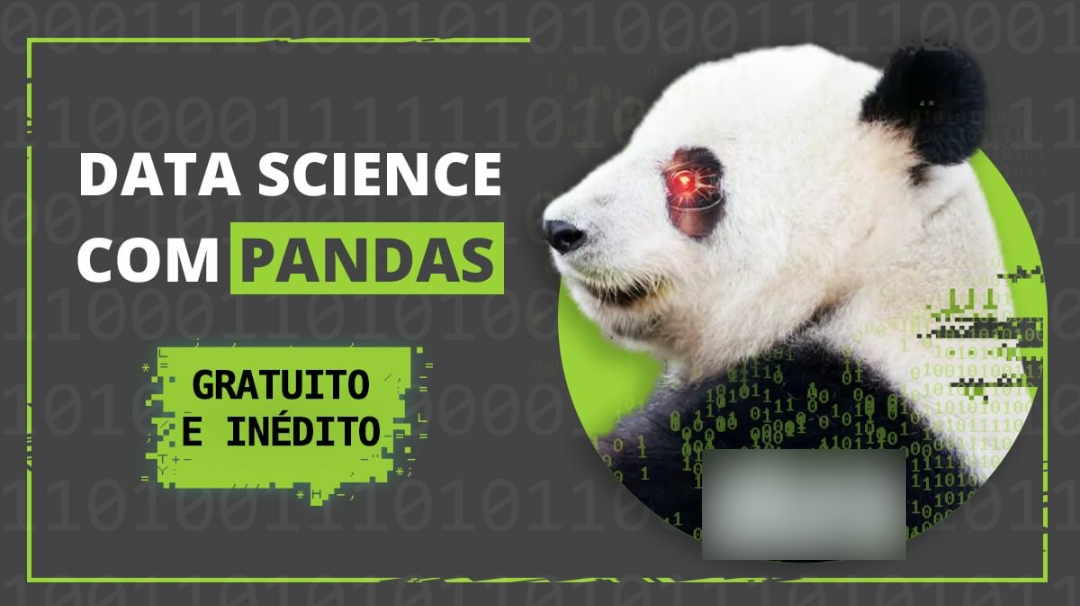
\includegraphics[width=0.45\textwidth]{eg_ds_1}\hfill
	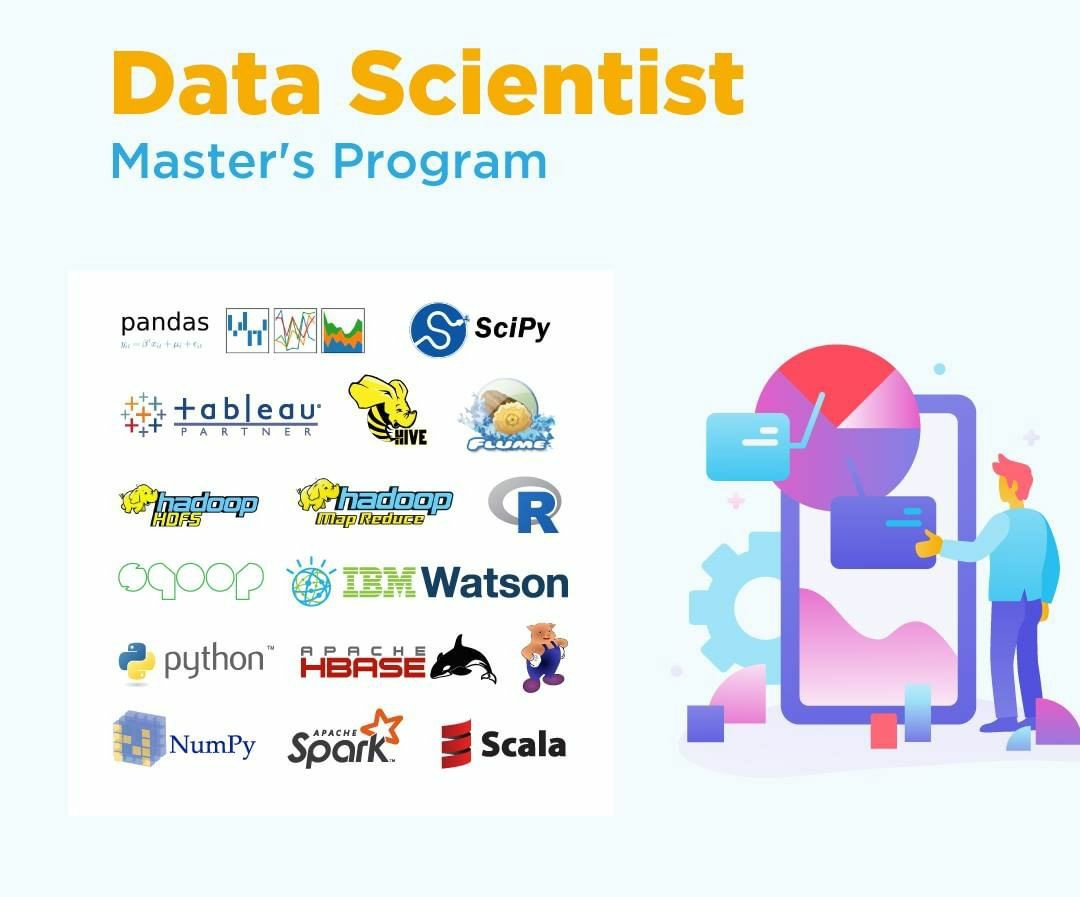
\includegraphics[width=0.45\textwidth]{eg_ds_2}

	\caption{Anúncios de cursos livres de ciência de dados.}
	\label{fig:cursos}
\end{figure}

Porém, como esses cursos visam o mercado de trabalho, em geral a divulgação deles enfatiza não os conhecimentos, competências e habilidades que um cientista de dados precisa, mas sim as ferramentas e algoritmos utilizados por eles e que são frequentemente mencionados em vagas de emprego.
A Figura~\ref{fig:cursos} ilustra isso: ela apresenta a propaganda de dois cursos, oferecidos na rede social Instagram.
Em ambos o foco é linguagens de programação (Python, Scala e R), ferramentas de \foreign{Big Data} (Spark, Hadoop \etc), aplicativos (Tableau) e bibliotecas (Pandas, SciPy \etc).

Embora o domínio dessas ferramentas seja necessário, ele não é suficiente para um cientista de dados de fato produzir conhecimento acionável.
Para isso são necessários, por exemplo, métodos de pesquisa, engenharia de dados, inferência estatística, dentre outros \cite[p.~15]{CF-DS-Release2019}.

Argumentamos, então, que a ênfase em ferramentas, linguagens \etc na \emph{divulgação} desses cursos esmorece, aos olhos dos alunos, a importância das habilidades e competências, haja vista que sua relação com as vagas de emprego não são tão explícitas como as linguages e ferramentas.